\section{Results}

The experiment results are presented as a chart\ref{fig:Results} containing the amount of 
points each agent was able to get while playing against the other agents. The agents are
RandomAgent, GreedyAgent, RLAgent.

\begin{figure}[h]
	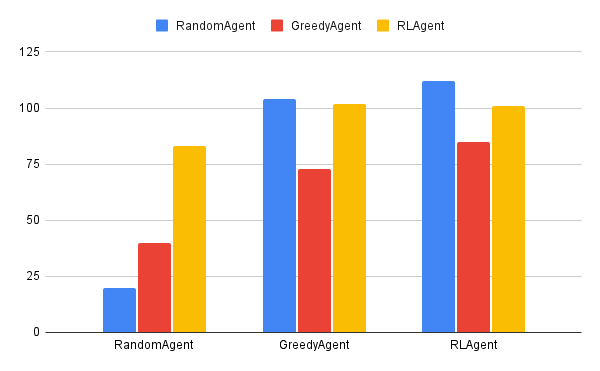
\includegraphics[width=\linewidth]{figures/chart}
	\caption{Experiment results. On the x-axis are the agents (starting players) being evaluated and on the y-axis the average amount of points earned during the experiments.}
	\label{fig:Results}
\end{figure}

The above mentioned results show that the engine's performance issues heavily
impacted the ability of the agent based on reinforcement learning to learn the game.
Based on this results team decided the next steps should be to improve the engine's
throughput as to increase the learning rate of the agent.
